\documentclass[letterpaper,10pt,titlepage]{article}

\usepackage{graphicx}                                        
\usepackage{amssymb}                                         
\usepackage{amsmath}                                         
\usepackage{amsthm}                                          

\usepackage{alltt}                                           
\usepackage{float}
\usepackage{color}
\usepackage{url}

%\usepackage{balance}
%\usepackage[TABBOTCAP, tight]{subfigure}
%\usepackage{enumitem}
\usepackage{pstricks, pst-node}

\usepackage{geometry}
\geometry{textheight=9in, textwidth=6.5in}

%random comment

\newcommand{\cred}[1]{{\color{red}#1}}
\newcommand{\cblue}[1]{{\color{blue}#1}}

\usepackage{hyperref}
\usepackage{geometry}

\def\name{Jacob Branaugh, Brenn Kucey}

%% The following metadata will show up in the PDF properties
\hypersetup{
  colorlinks = true,
  urlcolor = black,
  pdfauthor = {\name},
  pdfkeywords = {cs472 ``computer architecture'' clements ``chapter 3''},
  pdftitle = {CS 472: Homework 3},
  pdfsubject = {CS 472: Homework 3},
  pdfpagemode = UseNone
}

\begin{document}
\hfill \name

\hfill \today

\hfill CS 472 HW 3

\begin{enumerate}
	\item[(3.1)] Why is the program counter a \textit{pointer} and not a
		\textit{counter}?
	\item[\textbullet] If the program counter was a \textit{counter}, the instructions
		would have to be sequential. Since the program counter is a
		\textit{pointer}, the instructions can be located in any order since the
		PC simply gets the next address, enabling branching.

	\item[(3.2)] Explain the function of the following registers in a CPU:
	\begin{enumerate}
		\item[-] PC (program counter): The PC holds the address of the
			\textit{next} instruction to be fetched from memory
		\item[-] MAR (memory address register): the MAR holds the address of the
			memory location that is being accessed for reading/writing during 
			the current execute cycle
		\item[-] MBR (memory buffer register): the MBR holds the data that was
			read from or is about to be written to the location pointed to by
			the address in the MAR
		\item[-] IR (instruction register): the IR holds the instruction being
			currently executed
	\end{enumerate}

	\item[(3.3)] For each of the following 6-bit operations, calculate the values of
		the C, Z, V, and N flags.
		\\
		\\
		%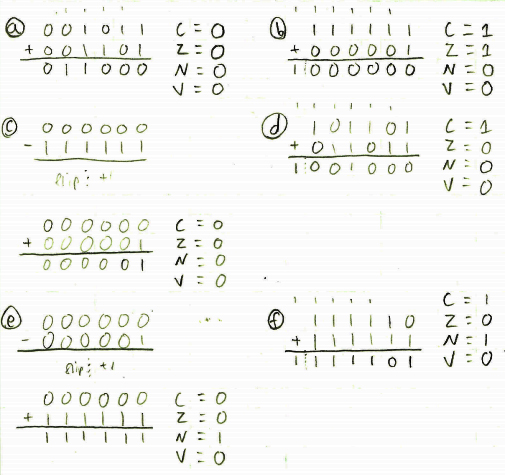
\includegraphics{problem3.jpg}

	\item[(3.10)] Why does the ARM provide a reverse subtract instruction \textit{RSB
		r0, r1, r2} that implements \textit{[r0] = [r2] - [r1]} when the normal
		subtraction instruction \textit{SUB  r0, r2, r1} will do exactly the same
		job?
	\item[\textbullet] Both operations only allow the last operand to be a flexible
		value. Flexible operands can be constants or registers with applied 
		shifts, instead of just registers. In this example, SUB allows r1 to be 
		flexible, while RSB allows r2 to be flexible. 

	\item[(3.17)] ARM instructions have a 12-bit literal. Instead of permitting a word
		in the range 0 to $2^{12}$-1, the ARM uses an 8-bit format for the integer
		and a 4-bit alignment field that allows the integer to be shifted in steps
		of 2. What are the advantages and disadvantages of this mechanism in
		comparison with a straight 12-bit integer?
	\item[\textbullet] The advantage is that the form is $(8-bit) \times  2^{4-bit}$ 
		allows for numbers larger than $2^{12}$-1. The disadvantage is that
		not all numbers between 255 and $255 \times 2^{15}$ cannot be represented 
		because not all numbers are multiples of this form.

%\item[(2.17)] What is the decimal equivalent of the 32-bit IEEE floating point value
%	CC4C0000?
%	\item[\textbullet] The following are the components of this floating point value:
%  \begin{enumerate}
%    \item[-] Sign = 1 (negative)
%    \item[-] Exponent = 10011000 = 152 - 127 = {\large\textit{\textbf{25}}}
%    \item[-] Significand = 1001100...0 = $\frac{1}{2}$ + $\frac{1}{16}$ + $\frac{1}{32}$ =
%	    $\frac{19}{32}$ = {\large\textit{\textbf{0.59375}}}
%    \item[-] Decimal number = $-1.59375 \times 2^{25}$ =
%	    {\large\textit{\textbf{-53477376}}} 
%  \end{enumerate}
%
%\item[(2.22)] What is the difference between a \textit{truncation} error and a
%	\textit{rounding} error?
%  \item[\textbullet] A truncation error is when bits are cut off of the end (which always
%	results in a round-down). A rounding error is when a number is either rounded up
%	or down based on whether the unwanted bits are greater than/equal to .5 or less
%	than .5, respectively. Both errors happen due to significant figure requirements.
%
%\item[2.40] Draw a truth table for the circuit below and explain what it does:
%  \item[\textbullet] This circuit is logically equivalent to an XOR. \\
%    \\
%    \begin{tabular}{ c c | c }
%	    A & B & C \\
%	    \hline
%	    0 & 0 & 0 \\
%	    0 & 1 & 1 \\
%	    1 & 0 & 1 \\
%	    1 & 1 & 0 \\
%    \end{tabular}
%
%\item[2.45] It is possible to have n-input AND, OR, NAND, and NOR gates, where n > 2. Can
%	you have an n-input XOR gate for n > 2? Explain your answer with a truth table.
%  \item[\textbullet] No, XOR gates can only have 2 inputs. An XOR gate with more than 2
%	  inputs can be representented with multiple 2 input XOR gates.

\end{enumerate}

\end{document}
